\documentclass[review]{elsarticle}
\usepackage[utf8]{vietnam}
\setlength{\parskip}{10pt}
%\usepackage[pdftex]{graphicx}
%\usepackage[font=footnotesize]{caption}

\usepackage{mwe}    % loads »blindtext« and »graphicx«
\usepackage{subfig}
\usepackage{float}

\usepackage{lineno,hyperref}
\modulolinenumbers[5]

\journal{Journal of \LaTeX\ Templates}

%%%%%%%%%%%%%%%%%%%%%%%
%% Elsevier bibliography styles
%%%%%%%%%%%%%%%%%%%%%%%
%% To change the style, put a % in front of the second line of the current style and
%% remove the % from the second line of the style you would like to use.
%%%%%%%%%%%%%%%%%%%%%%%

%% Numbered
%\bibliographystyle{model1-num-names}

%% Numbered without titles
%\bibliographystyle{model1a-num-names}

%% Harvard
%\bibliographystyle{model2-names.bst}\biboptions{authoryear}

%% Vancouver numbered
%\usepackage{numcompress}\bibliographystyle{model3-num-names}

%% Vancouver name/year
%\usepackage{numcompress}\bibliographystyle{model4-names}\biboptions{authoryear}

%% APA style
%\bibliographystyle{model5-names}\biboptions{authoryear}

%% AMA style
%\usepackage{numcompress}\bibliographystyle{model6-num-names}

%% `Elsevier LaTeX' style
\bibliographystyle{elsarticle-num}
%%%%%%%%%%%%%%%%%%%%%%%

\begin{document}

\begin{frontmatter}

\title{Pseudo-3D Trajectories: An Effective Approach for Motion Representation in Depth Data}

%% Group authors per affiliation:
\author{Chien-Quang LE}
\address{The Graduate University for Advanced Studies}

%% or include affiliations in footnotes:
\author{Duy-Dinh LE}
\address{National Institute of Informatics}

\author{Shin'ichi Satoh}
\address{National Institute of Informatics}


\begin{abstract}
Leveraging the motion information of trajectories shows the effectiveness to the human action recognition in 2D video. However, the issue is that this approach direction is effective or not when represents motions in 3D video is not still answered. In this paper, we will deal with this issue by conducting experiments based on 2D trajectory features to present motion information from one 3D video representation. Beside, in order to ensure including depth information, we propose a method based on compensating motion information from other representations. Evaluated on the benchmark datasets, our method significantly outperforms the 3D SoA methods.
\end{abstract}

\begin{keyword}
\texttt{Trajectory}\sep action recognition\sep depth\sep feature representation
%\MSC[2010] 00-01\sep  99-00
\end{keyword}

\end{frontmatter}

\linenumbers

\section{Introduction}

\paragraph{Background and Challenges} Gần đây, với sự phát triển của RGB-D camera như Kinect, depth data đã mở ra nhiều hướng nghiên cứu tiềm năng cho bài toán Human Action Recognition. So sánh với intensity images thông thường, depth maps hỗ trợ nhiều advantages hơn. Ví dụ, depth maps cung cấp các thông tin về shape rõ ràng hơn so với intensity images. Hơn thế nữa, depth data ít bị ảnh hưởng bởi những thay đổi của ánh sáng. Tuy nhiên, các phương pháp dựa trên intensity liệu có hiệu quả trên depth data hay không vẫn chưa được quan tâm nhiều.

\paragraph{Existing approaches and drawbacks} Trong bài toán action recognition, để adapt các phương pháp dựa trên intensity cho depth data có 2 yếu tố chính. Thứ nhất, để capture motion information hiệu quả việc chọn lựa a robust feature representation là rất quan trọng. Thứ hai, để đảm bảo motion là đầy đủ thông tin trong depth video, việc bổ sung thông tin depth vào feature representation là yêu cầu không thể thiếu. Tuy nhiên, các phương pháp được đề xuất gần đây vẫn chưa hội tụ đủ 2 yếu tố này. Một số phương pháp như [DMM-HOG, DSTIP-DCSF] xem xét depth value như là intensity value và adapt các intensity-based techniques. Mặc dù, chúng có thể đạt được những kết quả hợp lý, nhưng tất cả chúng đều phải đối mặt với nhiều hạn chế. [DMM-HOG] có thể tận dụng thông tin depth từ các phép chiếu của depth maps. Nhưng its feature representation dựa trên global motion như HOG sẽ dễ gây nhầm lẫn bởi những similar postures. [DSTIP-DCSF] có thể đảm bảo depth information trong việc tính toán features. Nhưng cách tiếp cận này không đảm bảo được sự tin cậy khi extract các local points, do bởi textureless data and depth noise. Ngoài hướng tiếp cận trên, các phương pháp như [LOP, HON4D] chỉ tập trung khai thác depth information nên không tận dụng được sức mạnh của các intensity-based features. Do đó, hướng nghiên cứu của chúng tôi là propose một phương pháp có thể đáp ứng đầy đủ cả 2 yếu tố nêu trên.

\paragraph{Proposal, Idea and Steps}Trong bài báo này, chúng tôi sử dụng một feature representation dựa trên dense trajectories của [Heng Wang], do bởi hiệu quả của cách tiếp cận này trong nhiều bài toán, including activity recognition and multimedia event detection. Các trajectories thu được bằng cách tracking các sampled points densely sử dụng optical flow fields. Sau khi extract trajectories, các trajectory-aligned descriptors sẽ được adopted. Sau đó, features tính toán được từ các descriptors này sẽ được sử dụng cho việc biểu diễn motion information trong video.

Tuy nhiên, việc thiếu sót depth information trong feature representation có thể gây ra các trường hợp bị confused, như được chỉ ra trong Figure \ref{subfig-1:FrontView}. Do đó, để đảm bảo việc không bỏ sót thông tin depth, ý tưởng cơ bản là combine thông tin chuyển động từ nhiều góc nhìn khác nhau. Các biểu diễn từ nhiều góc nhìn có thể đạt được bằng cách chiếu depth maps lên trên các mặt phẳng tương ứng. Việc chiếu này dễ dàng thực hiện được bởi những thuận lợi mà depth data mang lại.

\begin{figure}[H]
	\begin{center}
		\subfloat[From front view\label{subfig-1:FrontView}]{ %
			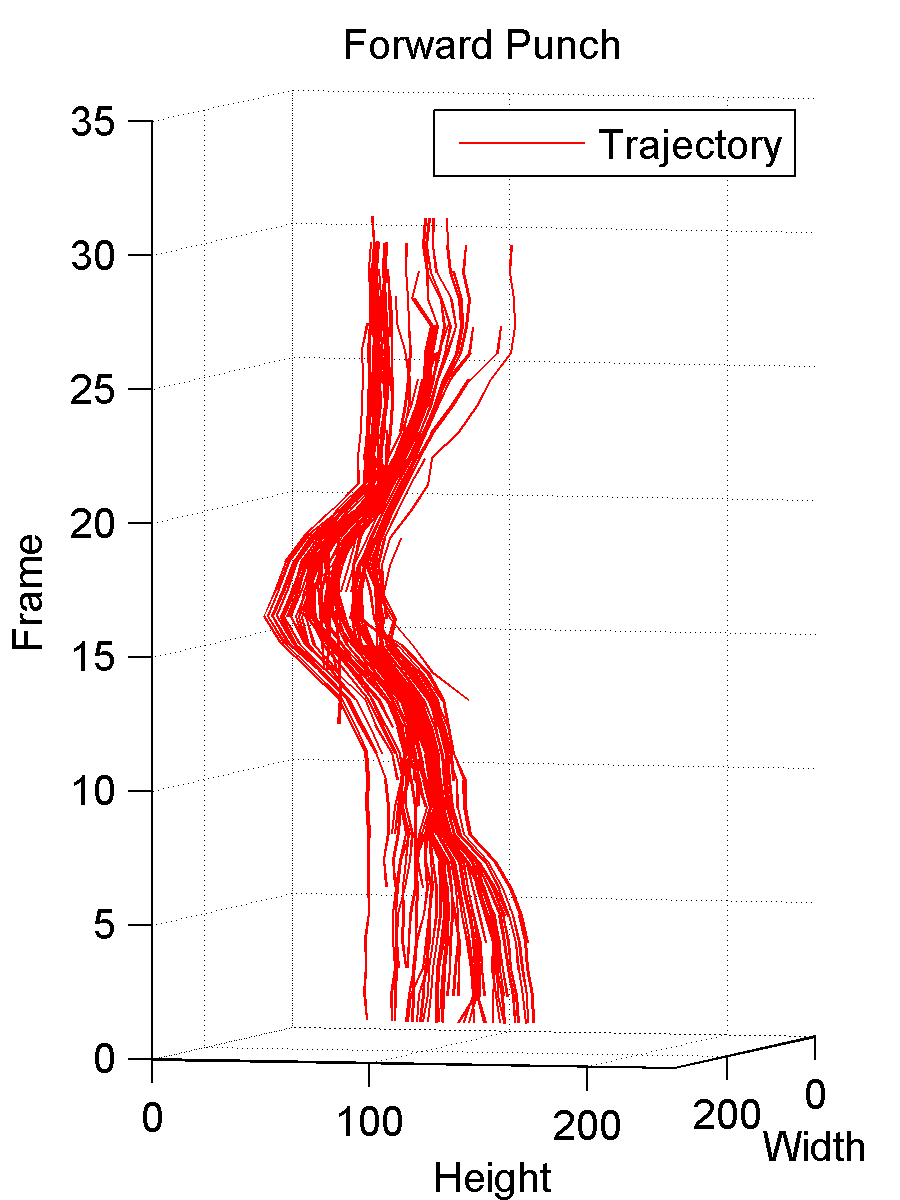
\includegraphics[scale=0.5]{ForwardPunch_FRONT.png}
			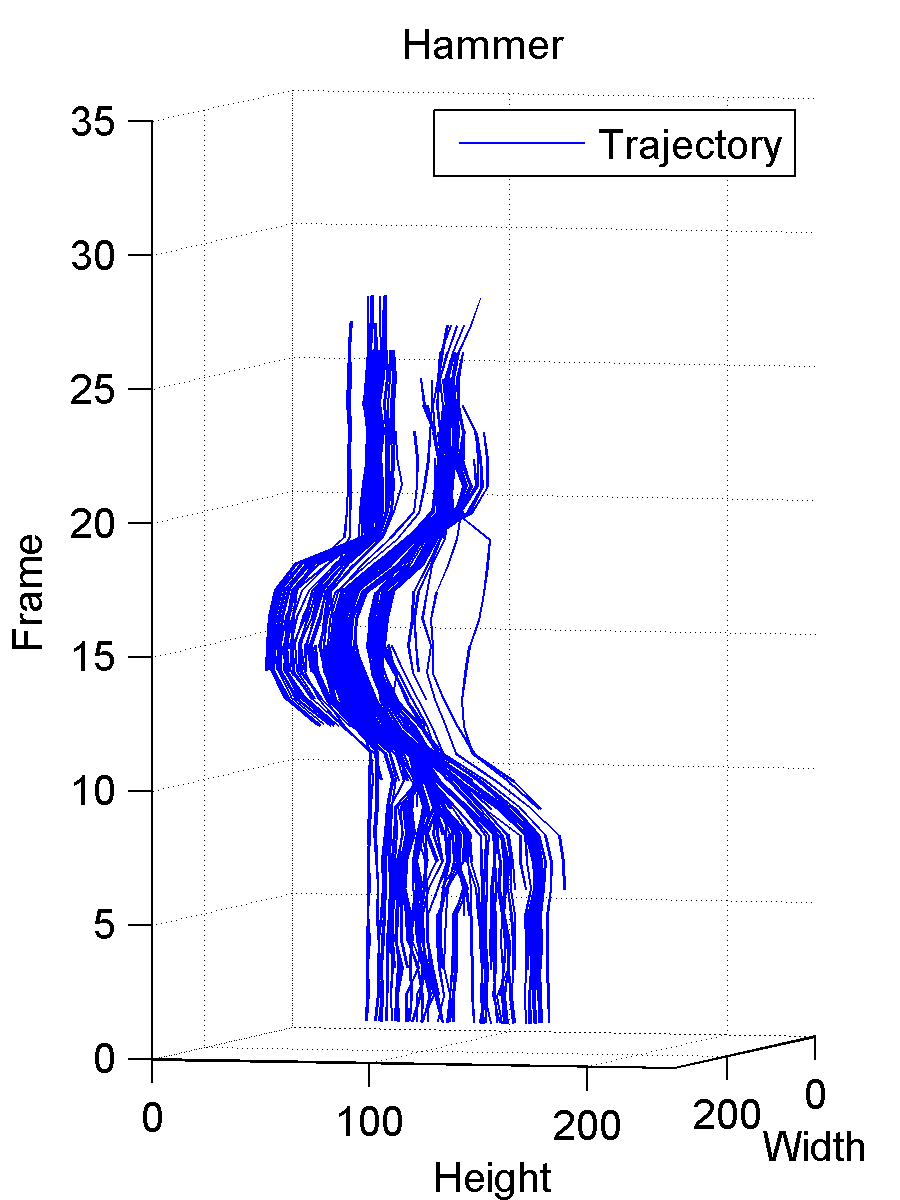
\includegraphics[scale=0.5]{Hammer_FRONT.png}
		}
	\end{center}
	\begin{center}
		\subfloat[From side view\label{subfig-2:SideView}]{ %
			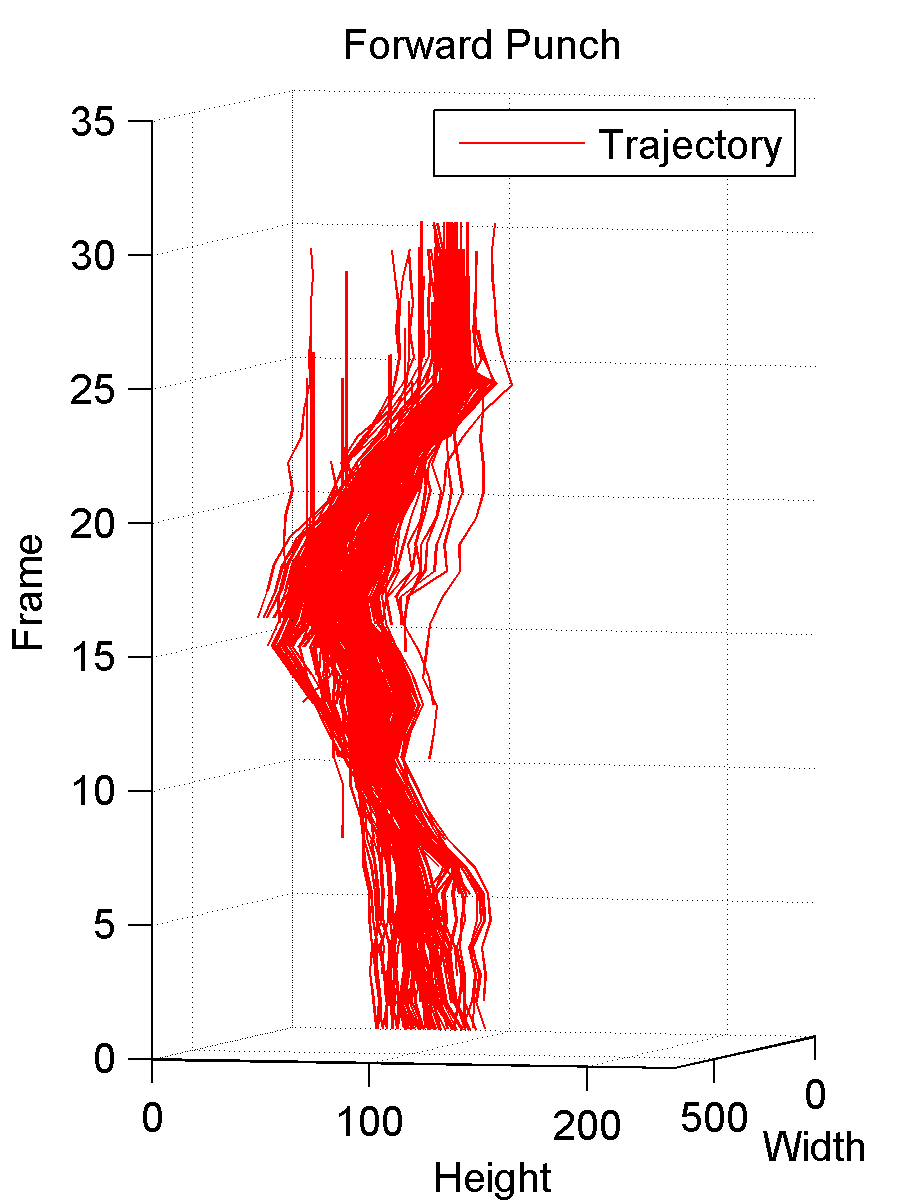
\includegraphics[scale=0.5]{ForwardPunch_SIDE.png}
			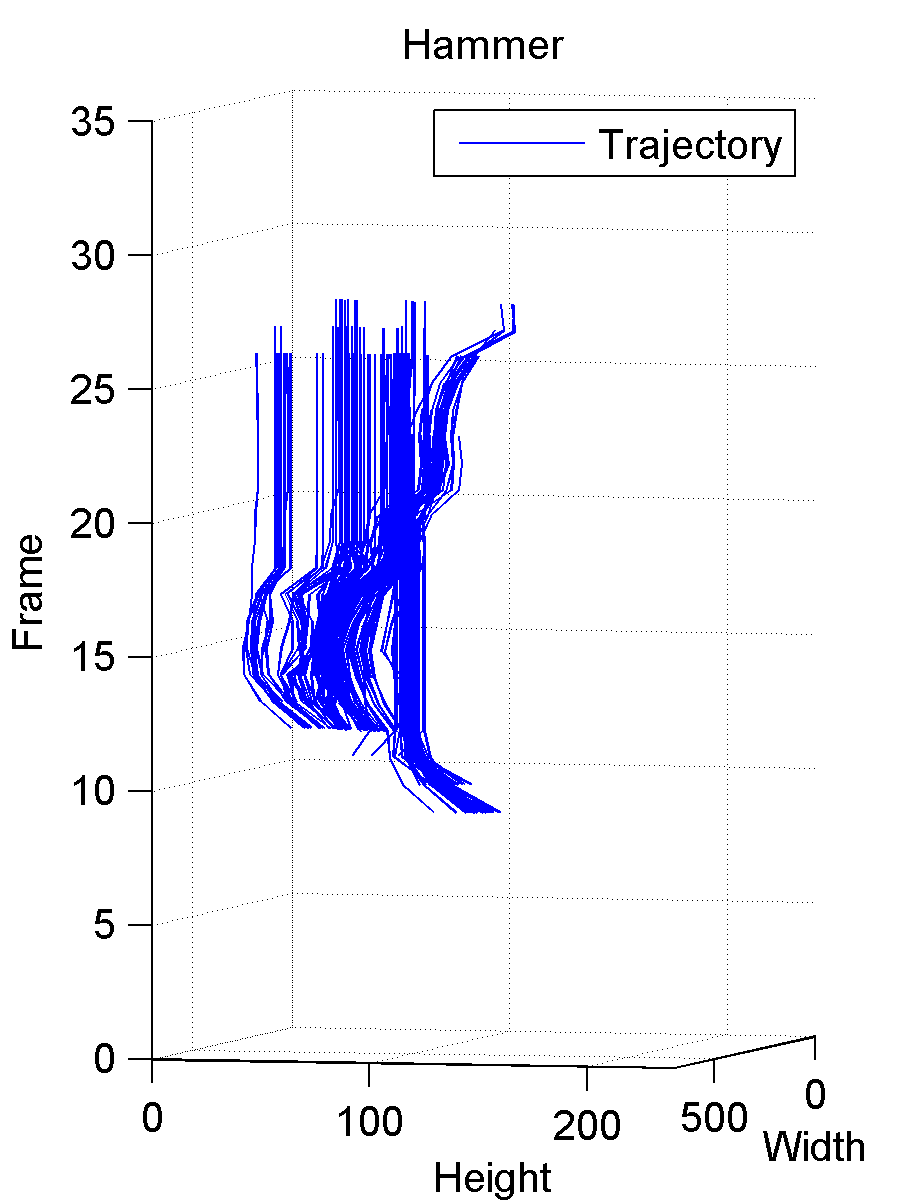
\includegraphics[scale=0.5]{Hammer_SIDE.png}
		}
	\end{center}
	\begin{center}
		\subfloat[From top view\label{subfig-3:TopView}]{ %
			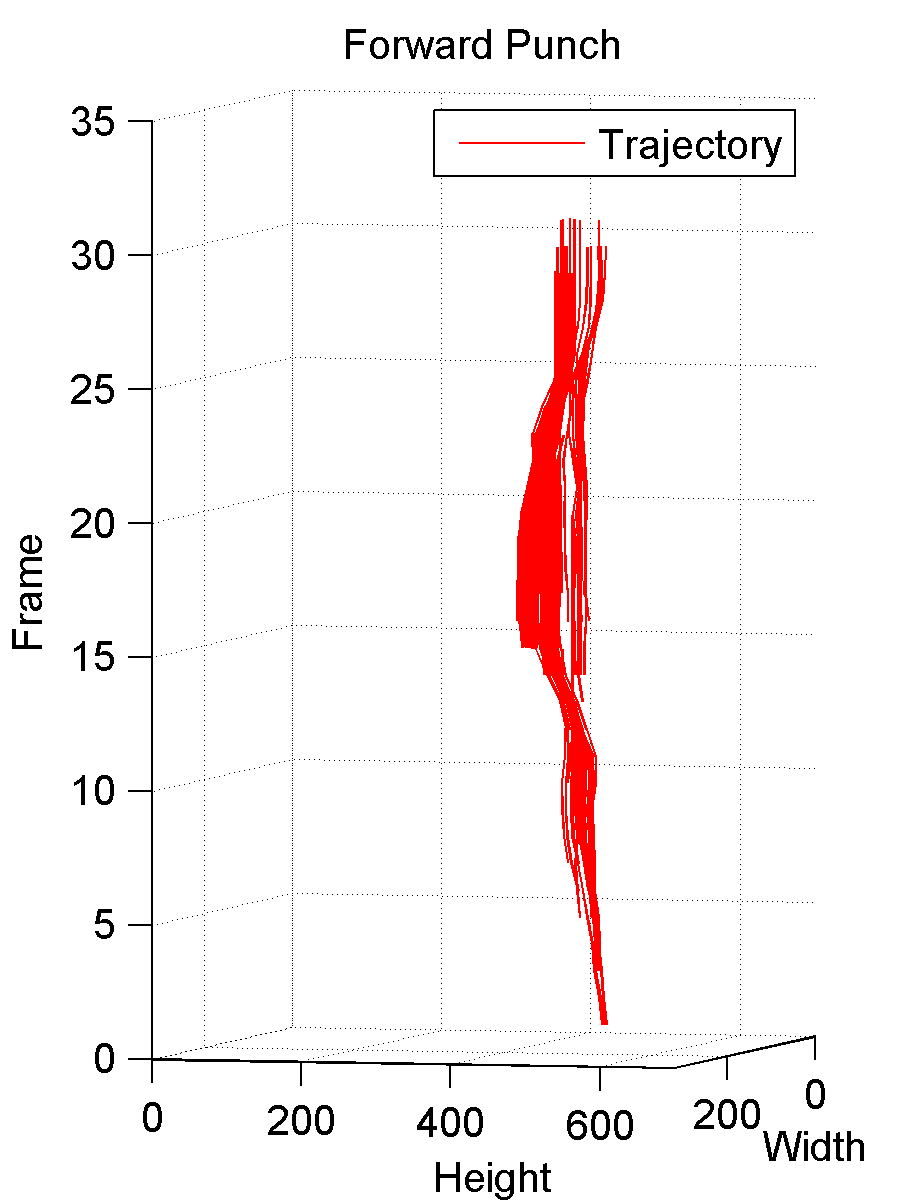
\includegraphics[scale=0.5]{ForwardPunch_TOP.png}
			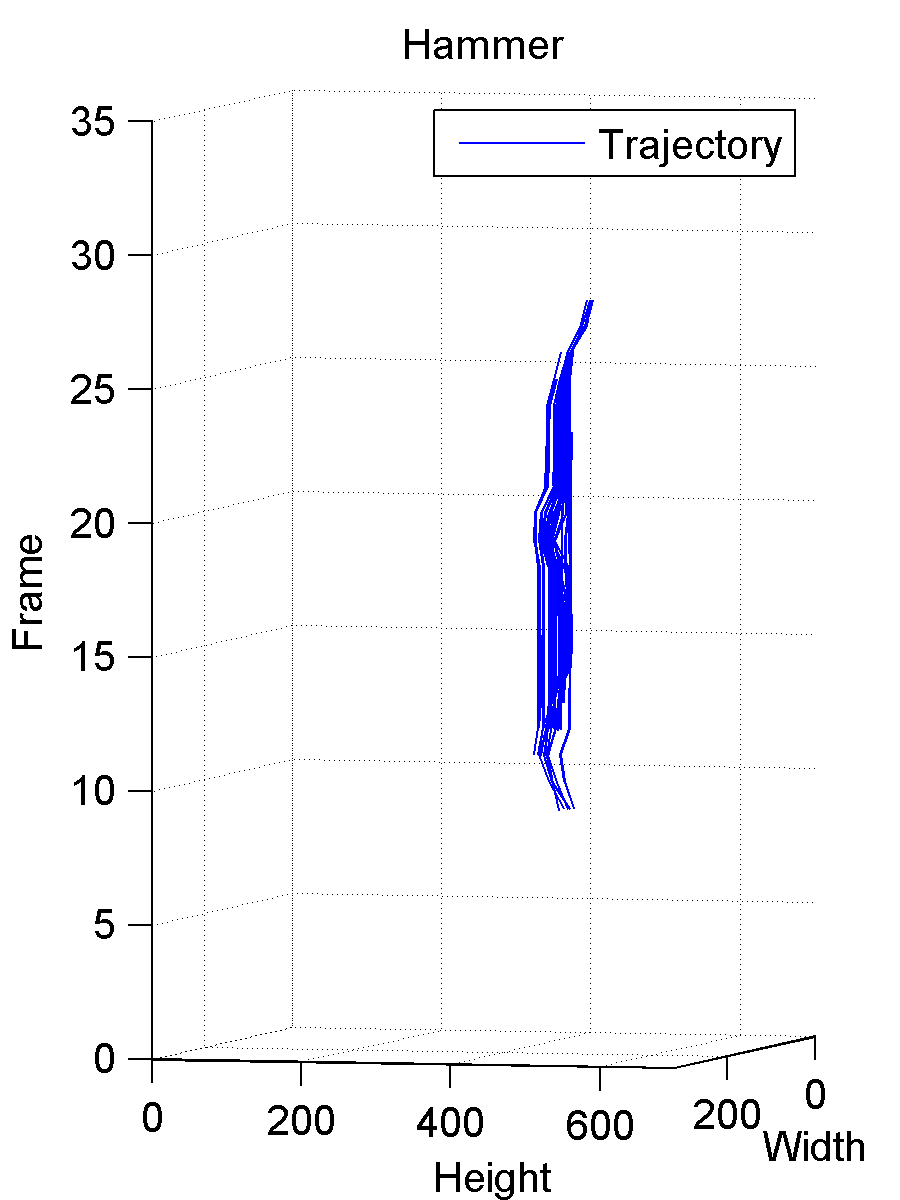
\includegraphics[scale=0.5]{Hammer_TOP.png}
		}
	\end{center}
	\caption{\label{fig:Illustration}Minh họa sự tương tự giữa phần lớn các Trajectories của 2 actions: Forward Punch \& Hammer.}
\end{figure}

\paragraph{Experiments and Results}Chúng tôi tiến hành các experiments trên challenging benchmark datasets, các kết quả thí nghiệm chỉ ra rằng phương pháp của chúng tôi đánh bại the SoA methods trên depth data. Các kết quả này đã cho thấy những contributions của our method: (1) We propose an adaptive method for 3D video representation by using 2D features. (2) We thực hiện comprehensive experiments on the state-of-the-art MSR Action 3D dataset and show that our method is the best when compared with the state-of-the-art 3D methods.

\paragraph{Paper structure}After a brief review of the related work in Section 2, the proposed method is described in Section 3. Section 4 presents the experimental results and their concerned discussions. The summaries of our work are given in Section 5.

\section{Related Works}

Tìm hiểu các thành phần của một hệ thống HAR hiện là một trong những hướng nghiên cứu quan trọng của CV.
Feature representation là 1 trong số các thành phần thu hút được sự chú ý của cộng đồng nghiên cứu.

\paragraph{Works trích chọn features từ depth data}
- Hướng xem depth value như intensity value.
- Hướng sử dụng real depth value và skeleton information.

\paragraph{Điểm khác biệt của phương pháp hiện tại với các phương pháp trước}
- Hướng sử dụng 2d trajectories cho 3d data.

\paragraph{Works in combining many types of features and sự khác biệt với our work}
- Works gần đây sử dụng early fusion sheme.
- Our method sử dụng late fusion sheme.

\section{Proposed Method}

\subsection{Dense trajectories}
- Giới thiệu khái quát về dense trajectories
- Giới thiệu sơ lược về các descriptors: HOG, HOF, MBH

\subsection{Pseudo-3D trajectory-based approach for motion feature}
- Hình - Illustration of proposed method
- Hình - Framework overview for our system
- Step 1 - Project depth maps onto orthogonal planes
- Step 2 - Extract dense trajectories from scaled videos
- Step 3 - Fuse motion information from different views

\section{Experimental Settings}

\subsection{Dataset}
- Giới thiệu về MSR Action 3D dataset
- Table - 20 actions
- Table - 3 subsets
- Mô tả đặc điểm của 3 subsets
- Settings trong thí nghiệm

\subsection{Evaluation Method}
- Sử dụng thư viện online để extract DT
- Mô tả các settings trong framework: Number of codewords, assignment method, BoW model, SVM ở 2 pha phân lớp
- Thư viện libsvm
- Đánh giá dựa trên accuracy

\section{Experimental Results}

\subsection{Recognize actions from single-view}
- Mô tả thí nghiệm trên 1 view
- Table - Kết quả trên front view
- Nhận xét các trường hợp bị confused, lý giải dựa trên trajectory shape
- Figure - Ví dụ về các trường hợp bị confused

\subsection{Fuse motion information from all views}
- Mô tả thí nghiệm trên 3 view
- Table - So sánh với SoA
- Đánh giá lại các trường hợp bị confused
- Figure - Ví dụ về trajectories trên các views khác

\subsection{The impact of our method on descriptors}
- Mô tả thí nghiệm trên 3 descriptors: HOG, HOF, MBH
- Nhận xét trước khi fusion
- Nhận xét sau khi khi fusion:
    + Compensate information
    + Keep salient information

\section{Conclusions}

\paragraph{Tóm tắt our work}

\paragraph{Đề xuất cho future work}



\section*{References}

\paragraph{Cách cite ref}Here are two sample references: \cite{Feynman1963118,Dirac1953888}.

\bibliography{mybibfile}

\end{document}